\section{Method}

Our research involved human subjects, and our experimental procedures were approved by an Institutional Review Board. We recruited 15 subjects to participate in our study, all of whom were UC Berkeley undergraduate or graduate students. Each subject met with investigators in a quiet, closed room for two 40-50 minute sessions on two separate days. We briefed subjects on the objective of the study, fitted them with a Neurosky MindSet headset, and provided instructions for completing each task. As the subjects performed each task, we recorded readings from the headset (i.e., difference of potential and power spectrum every half second).

\subsection{Tasks}

% TODO: steal from passthoguhts

\subsection{Signal extraction}

Before analyzing the data, we compute the power spectrum data using a fast Fourier transform \textcolor{red}{I think this is done by the software}. We then compress the data in the temporal dimension, taking the middle \textit{n} seconds of the recording, where \textit{n} is {0.5, 1, 2, 3, 4, 5, 6, 7, 8, 9}. 

%TODO: publishable-ify stuff below

%---------------

Following your questions on how I generated the input for the classifier from Benjamin's raw data, I could recall what input I prepared. It's quite simple and robust, and now I see better why it seems to classify quite well, maybe better that other methods.

The Neurosky software (on John's netbook) computes a power spectrum every half second. Then, the maximum frequency is 256Hz (because the maximum sampling rate of Neurosky hardware is 512Hz). The power spectrum is computed with discrete bins of 1/4 Hz. Each bin represents the intensity of activation of a frequency range (e.g., between 1 and 1.25 Hz) in a half-second time window. There are therefore 1024 values reported for one power spectrum. Our samples are more or less 10 seconds, which means around 20 power spectra computed per sample. Based on the signal quality also recorded some power spectra are removed (Benjamin knows the exact filtering method).

The spirit of the method developed consists in two steps : (i) build a statistical significance out of the n power spectra produced in each sample, and (ii) "compress" the information to have vector of arbitrary size < 1024.

For each bin of 1/4 Hz, we can compute a median value out of the n power spectra generated for one sample.  We obtain a discrete probability density function (pdf) with each bin being the median of the corresponding bins in the n power spectra. At this stage, we have a discrete pdf of 1024 bins for the whole sample. This method is called a ``stacking" of several probability density functions into one representing the statistical average of all the others.

However, for a classifier, it is desirable to have less values (i.e., of the order of 10 to 100). But we don't want to lose information on the whole pdf. Binning the pdf is a simple way to ``compress" the information contained in the original power spectrum. The basic idea is to take the median of several bins. For instance, four contiguous bins (1-1.25,1.25-1.5,1.5-1.75,1.75-2) have the values (4,4,5,5) the value resulting from combining these values into one bin would be 4.5. The pdf is heavy-tailed and it is desirable to arrange the ``compression" bins in a way it provides relevant information on the whole distribution. One way to do this efficiently is to arrange the compression bins in a logarithmic fashion.

\textcolor{red}{\bf [I think here is the originality of the method: we take all the power spectrum with one advantage and one disadvantage. The advantage is that we have a much larger spectrum to characterize and classify tasks, at the cost of probably more pollution from non-EEG signal from the environment, from muscles, etc.]}

% \begin{figure}
% \begin{center}
% 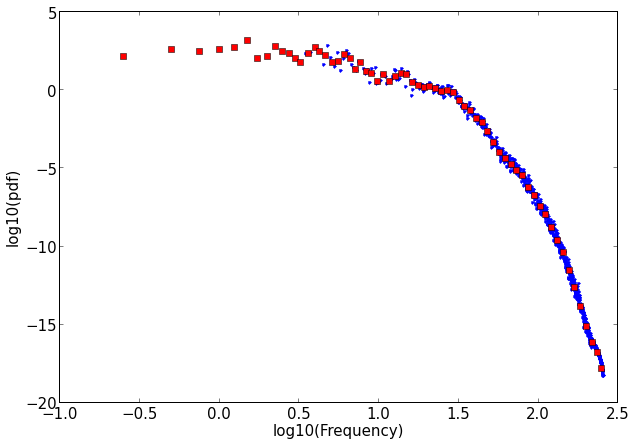
\includegraphics[width=5in]{Figures/binned_EEGpowerspectrum.png}
% \caption{Binned power spectrum}
% \label{binnedEEGpowerspec}
% \end{center}
% \end{figure}

\textcolor{red}{\bf [About here, a short pitch on pink noise is required to set the stage of the great method, and to justify the log log binning]}

Figure \ref{binnedEEGpowerspec} shows, in double logarithmic scale, the original 1024 bins (blue dots) of the pdf obtained from averaging the n power spectra of one sample, and the resulting "compressed"  pdf with 100 log-bins. As we can see, the log-binning preserves very well the structure of the pdf.

In summary, we have built a probability density function of brain frequencies as captured by the Neurosky hardware, from the n power spectra of each sample. We have then used a log-binning method to reduce the 1024 bins from the original power spectrum to an arbitrary smaller number of log-bins (e.g., 100 log-bins on the Figure). This method makes a sort of statistical averaging by stacking, and then ``compresses" the result in way that it is easy to use in a classifier.

{\bf NB:} I believe that the classifier does well because it can efficiently capture the overall level of activity for all log-bins, but also more local deviations. On the figure, we can see some local peaks mostly between $10^1$ and $10^1.5$, but in all other parts of the pdf though in a less visible way. I believe these deviations are quite unique and can make the difference in the classifier. We should indeed check this further if we want to understand to origins of the good results.

{\bf Side note:} one way to investigate further would be to see indeed to what extent the ``compression", i.e. the small number of log-bins, affects the quality of the classifier. Another quite promising further research direction, would be to determine the minimum number of n power spectra, which should be taken into account to reach a target level of correct classification. This would be useful to determine what should be the most adequate sample size for a certain level of identification. This level might of course vary as a function of subjects and tasks.

%-----------

Finally, we create a one-dimensional signal by flattening each bin in the time dimension, computing the mean magnitude of each bin over all readings in the recording. The resulting signal is a one-dimensional row vector with one entry for each each measured frequncy bin.

\textcolor{red}{\bf [Maybe a schema would be great to help the reader get the point quickly]}

From this point, we are equipped with a feature vector of arbitrary size and statistical relevance as an input for our classifier.

\subsection{Classifier}

Support vector machines (SVM) are a set of supervised machine learning methods that take labeled example data to create a model that can be used to predict the classes of unlabeled data. SVMs use a hyperplane (an n-dimensional construct in n+1 dimensional space) to draw discriminatory boundaries between classes. In contrast to linear discriminant analysis, which has a long history of use in BCIs, SVMs select the hyperplane that maximizes distance from the nearest training points, which has been shown to increase the model's generalizability \cite{burges_tutorial_1998}.  For more on SVM's in BCI: \cite{garrett_comparison_2003,grierson_better_2011} 

In this study, we use LinearSVC, \cite{fan_liblinear:_2008} a wrapper for LibLinear exposed in Python through the ScikitLearn library. \cite{pedregosa_scikit-learn:_2011} We chose LinearSVC primarily because its underlying C implementation is very performant, and because linear kernels performed as well or better than nonlinear ones in early experimentation, corroborating the findings of previous studies \cite{garrett_comparison_2003,lotte_review_2007} \textcolor{red}{Please provide evidence if you can}.  We use the default settings for LinearSVC - a C of 1.0, squared hinge loss function, and a tolerance parameter of of 1e-4. \textcolor{red}{You might want to explain what these parameters are, by e.g., providing the main formula of the LinearSVC.}


\subsection{Per-user calibration}

We conducted a simulated calibration step for each participant. For each subject, we generated every possible pair of two tasks and cross-validated our SVM seven times on that subject's recordings for those two tasks. We used ScikitLearn's built-in cross-validation toolkit, which was configured to perform each of the seven cross-validation steps using different splits of trial data in the training and testing sets. For every task pair processed, we recorded mean classification across all cross-validation trials. We repeated this calibration process for all users at every combination of recording length and (log-)bin size. 

As an additional performance audit, we timed our SVM at training time. We fit an SVM to all the data for two task-pairs from two randomly-selected subjects, and repeated this process ten thousand times at different bin sizes and different lengths. We report the minimum time of each ten thousand attempts. In order to establish a proper estimate, we time the SVM after all data has been loaded to memory, disregarding the time it takes to load the data from disk.

\textcolor{red}{[Is this time thing relevant in the sense that some situations really provide a significant gain compared to others?]}

% TODO: we should test at test-time also no?

